\section{L03-Trasformazioni}
Per variabile di stato si intende una grandezza che dipende dallo stato del sistema, viceversa variabili come il lavoro e il calore (che non sono di stato) non dipendono dallo stato del sistema, ma bensì dal percorso che hanno seguito per raggiungere quel determinato stato.
\subsection{Il lavoro termodinamico}
In un dispositivo cilindro-pistone, uno squilibrio di forze infinitesimo tra forze esterne e forza interna ($P \cdot A$) provoca uno spostamento infinitesimo del pistone a cui corrisponde un \textbf{lavoro}
\[
    \delta L^\rightarrow  = P A ds = P \cdot dV
\]
\begin{center}
    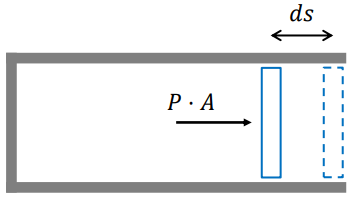
\includegraphics[height=3cm]{../L03/img1.PNG}
\end{center}
In termini di grandezze specifiche, la relazione diventa
\[
    \delta l^\rightarrow = P \cdot dv
\]
Quando il sistema evolve da uno stato \textbf{iniziale} (i) ad uno stato \textbf{finale} (f) attraverso una successione di \textbf{stati di equilibrio}, allora sarà possibile esprimere una legge, detta \textbf{equazione della trasformazione}, tra le variabili di stato $P$ e $v$ e la integrazione di $P dv$ rappresenterà il lavoro scambiato durante la trasformazione.\newline
Il lavoro termodinamico è dunque calcolabile come
\[
    l^\rightarrow = \int_{i}^{f}Pdv
\]
che è un integrale calcolabile solo se si conosce la funzione $P = P (v)$ detta equazione della trasformazione.
\subsubsection{Il lavoro termodinamico nelle trasformazioni reversibili e irreversibile}
Nel caso di trasformazione \textbf{reversibile} in un cilindro-pistone la pressione interna è sempre omogenea all'interno del cilindro.
\begin{center}
    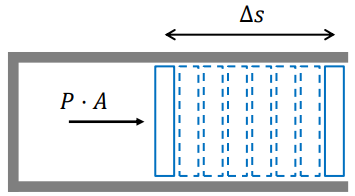
\includegraphics[height=2cm]{../L03/img2.PNG}
\end{center}
Nel caso di trasformazione \textbf{irreversibile} in un cilindro-pistone la pressione interna non è omogenea all'interno del cilindro. Quindi per ricavare la forza applicata al pistone si usa la pressione dell'ambiente esterno che agisce sul pistone.
\begin{center}
    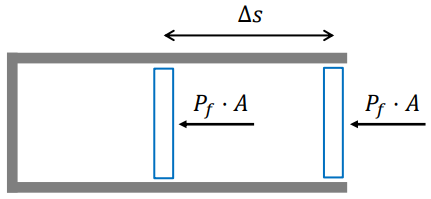
\includegraphics[height=2cm]{../L03/img3.PNG}
\end{center}
\ \newline
\newline
Solitamente il lavoro reversibile è maggiore del lavoro irreversibile, come si vede bene dal seguente grafico:
\begin{center}
    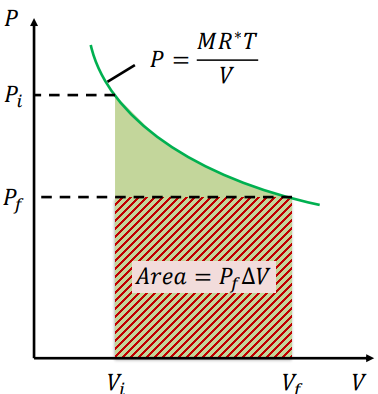
\includegraphics[height=5cm]{../L03/img4.PNG}
\end{center}
L'area verde insime all'area a linee rosse (cioè tutta quella sottesa alla curva) rappresenta il lavoro nel caso di trasformazione reversibile, la sola area a linee rosse rappresenta, invece, il lavoro nel caso di trasformazione irreversibile.
\subsubsection{Il lavoro termodinamico di un ciclo}
Un ciclo è un trasformazione che termina con lo stato iniziale. In funzione di come avviene il ciclo, orario o antiorario per esempio, avremo che il lavoro uscente dal sistema è positivo o negativo. Nel
piano $PV$ chiamiamo macchine a \textbf{ciclo diretto} (motrici) quelle che eseguono trasformazioni in senso orario, mentre chiameremo macchine a \textbf{ciclo inverso} (operatrici) quelle che eseguono trasformazioni in senso antiorario.
\begin{center}
    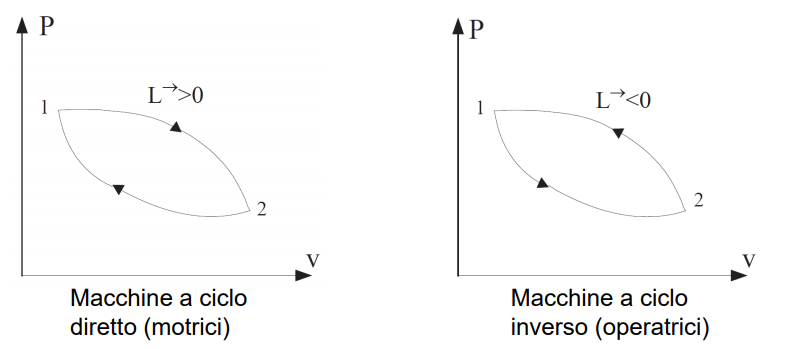
\includegraphics[height=3cm]{../L03/img5.PNG}
\end{center}
\subsection{Il calore}
\textbf{Capacità termica}: è il rapporto fra il calore fornito al sistema e la variazione di temperature del sistema stesso
\[
    C_x = \left(\frac{\delta Q^\leftarrow }{d T}\right)_x
\]
\textbf{Calore specifico}: è il rapporto tra la capacità termica del sistema e la sua massa
\[
    c_x = \frac{1}{M}\left(\frac{\delta Q^\leftarrow }{dT}\right)_x
\]
I calori specifici possono essere interpretati come \textbf{derivate parziali di funzioni termodinamiche}.\newline
\newline
Il pedice $x$ precisa la \textbf{trasformazione} lungo la quale viene scambiato il calore $\delta Q$. Vediamo i casi in cui $x$ è la pressione e il caso in cui è il volume.
\subsubsection{Calori specifici a volume costante $c_V$}
\[
    c_V =\frac{1}{M}\left(\frac{\delta Q^\leftarrow }{dT}\right)_V = \left(\frac{\delta q^\leftarrow }{dT}\right)_V
\]
Partendo dal primo principio della termodinamica e dalla definizione di lavoro data precedentemente si può scrivere che $\delta q^\leftarrow  = d u + Pdv$ e che quindi $\delta q^\leftarrow  = \left(\frac{\delta u}{\delta T}\right)_vdT + \left(\frac{\delta u}{\delta T}\right)_T dv + Pdv$, e proseguendo considerando il fatto che il volume è costante ricaviamo che $\delta q^\leftarrow  = \left(\frac{\delta u}{\delta T}\right)_VdT$, da cui ricaviamo che 
\[
    c_V = \left( \frac{\delta u}{\delta T} \right)_V
\]
Siccome è una \textbf{derivata di una funzione di stato}, può in generale essere espresso come funzione di una coppia di variabili termodinamiche (in particolare della coppia $T$,$P$):
\[
    c_V = c_V(T,P)
\]
\subsubsection{Calori specifici a pressione costante $c_P$}
\[
    c_P =\frac{1}{M}\left(\frac{\delta Q^\leftarrow }{dT}\right)_P = \left(\frac{\delta q^\leftarrow }{dT}\right)_P
\]
Per lavorare sul calore specifico a pressione costante dobbiamo introdurre la funzione di stato \textbf{entalpia}, che esprime la quantità di energia che un sistema può scambiare con l'ambiente ed è definita come
\[
    h = u + Pv
\]
Per le trasformazioni che avvengono a pressione costante, la variazione di entalpia è uguale al calore scambiato dal sistema con l'ambiente esterno. Col suo differenziale possiamo riscrivere il primo principio come $dh = du + vdP + Pdv$, da cui, ricordando che siamo a pressione costante, ricaviamo che $\delta q^\leftarrow = dh - vdP = \left(\frac{\delta h}{\delta T}\right)_P dT + \left(\frac{\delta h}{\delta T}\right)_T dP - vdP$, e quindi $\delta q^\leftarrow  =  \left(\frac{\delta h}{\delta T}\right)_P dT$, da cui ricaviamo che
\[
    c_P =  \left(\frac{\delta h}{\delta T}\right)_P
\]
Siccome è una \textbf{derivata di una funzione di stato}, può in generale essere espresso come funzione di una coppia di variabili termodinamiche (in particolare della coppia $T$,$P$): 
\[
    c_P = c_P(T,P)
\]
\subsubsection{$c_V$ e $c_P$ per i gas ideali}
Per un gas ideale la variazione di energia interna e l'entalpia sono funzioni della sola temperatura $u = u(T)$ e $h = h(T)$, per cui i calori specifici da derivate parziali diventano derivate esatte:
\[
    c_V = c_V(T) = \left(\frac{d u}{d T}\right)
\]
\[
    c_P = c_P(T) = \left( \frac{d h}{ d T}\right)
\]
Vale inoltre la \textbf{realzione di Mayer}
\[
    c_P = c_V + R^*
\]
\subsubsection{$c_V$ e $c_P$ per i gas perfetti}
Per i gas ideali i calori specifici dipendono dalla temperatura, ma questa relazione di dipendenza è molto debole, per cui in intervalli ristretti di temperatura i calori specifici si ritengono spesso costanti: in questo caso il gas viene definito \textbf{perfetto}.\newline
\newline
Per calcolare i calori specifici si usano le seguenti relazioni:
\begin{itemize}
    \item \textbf{Gas monoatomico} ($He$, $Ar$)
    \[
        c_v = \frac{3}{2}R^*; \;\;\;\;\;\;\;\;\;\;\;\;\;\;\;c_P = \frac{5}{2}R^*
    \]
    \item \textbf{Gas biatomico o poliatomico lineare}: ($N_2$, $O_2$, $CO_2$)
    \[
        c_v = \frac{5}{2}R^*; \;\;\;\;\;\;\;\;\;\;\;\;\;\;\;c_P = \frac{7}{2}R^*
    \]
    \item \textbf{Gas poliatomico non lineare}: ($CH_4$)
    \[
        c_v = \frac{6}{2}R^*; \;\;\;\;\;\;\;\;\;\;\;\;\;\;\;c_P = \frac{8}{2}R^*
    \]
\end{itemize}
\subsubsection{$c_V$ e $c_P$ per i liqudi (e solidi) incomprimibili ideali}
\[
    c_V = c_P = c(T)
\]
\subsubsection{$c_V$ e $c_P$ per i liqudi (e solidi) incomprimibili perfetti}
\[
    c_V = c_P = c = \text{costante}
\]
\subsection{Le trasformazioni politropiche}
Una \textbf{trasformazione politropica} è una trasformazione \textbf{quasi-statica}, cioè internamente reversibile, di un \textbf{gas ideale} per la quale $c_x = $ costante.\newline
\newline
Si definisce \textbf{indice della politropica}:
\[
    n = \frac{c_x-c_P}{c_x-c_V}
\]
e l' \textbf{equazione della politropica}:
\[
    Pv^n = \text{costante}
\]
\subsubsection{Trasformazione politropica per un gas ideale}
Per un gas ideale il valore di $n$ è calcolabile
\begin{center}
    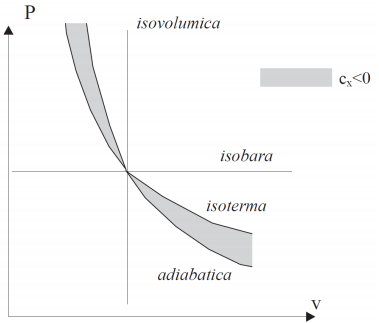
\includegraphics[height=3cm]{../L03/img6.PNG}
\end{center}
\subsubsection{Trasformazione politropica per un gas perfetto}
Per un gas perfetto il valore di $n$ è calcolabile
\begin{center}
    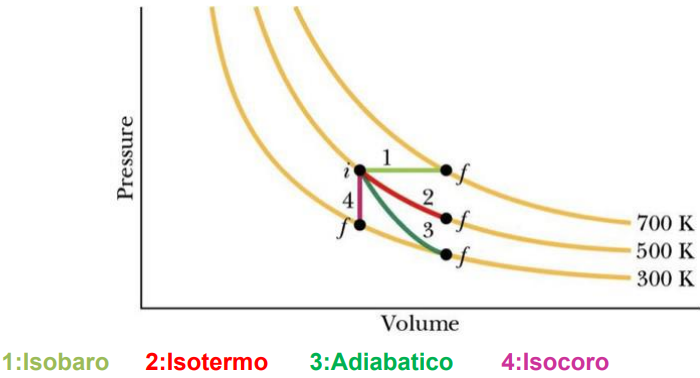
\includegraphics[height=3cm]{../L03/img7.PNG}
\end{center}
\subsubsection{Espressioni della politropica}
\[
    Pv^n = costante
\]
\[
    Tv^{n-1} = costante
\]
\[
    PT^{\frac{n}{1-n}} = costante
\]
\[
    Pvv^{n-1} = costante
\]
\[
    T\left(\frac{R^*T}{P}\right)^{n-1}= costante
\]
\[
    \frac{T^n}{P^{n-1}} = costante
\]
\subsubsection{Politropiche per trasformazioni elementari}
\begin{center}
    \begin{tabular}{ |c|c|c|c| } 
    \hline
    Trasformazione & $c_x$ & $n = \frac{c_x - x_P}{c_x - c_V}$ \\
    \hline
    Isoterma ($T = costante$) & $\pm \infty$ & $1$ \\ 
    Isocora ($v = costante$) & $c_V$ & $\pm \infty$\\ 
    Isobara ($P = costante$) & $c_P$ & $0$\\ 
    Adiabatica ($q = costante$) & $0$ & $k= \frac{c_P}{c_V}$\\ 
    \hline
    \end{tabular}
    \end{center}
\subsubsection{Lavoro di una generica politropica}
\begin{itemize}
    \item per $n\neq 1$ 
    \[
        l^\rightarrow = \frac{P_1 v_1}{n-1}\left[1- \left(\frac{v_1}{v_2}\right)^{n-1}\right]
    \]
    \[
        l^\rightarrow = \frac{P_1 v_1}{n-1}\left[1- \left(\frac{P_2}{P_1}\right)^{\frac{n-1}{n}}\right]
    \]
    \item per $n = 1$
    \[
        l^\rightarrow = P_1v_1 ln \frac{v_2}{v_1}
    \]
    \[
        l^\rightarrow = P_1 v_1 ln \frac{P_1}{P_2}
    \]
\end{itemize}
\subsubsection{Politropiche nel diagramma T-S}
In un diagramma T-S, l'\textbf{area sottesa dalla curva} rappresentativa di una trasformazione \textbf{internamente reversibile} è uguale al \textbf{calore} scambiato dal sistema nella trasformazione:
\[
    Q_{rev} = \int_{i}^{f}\delta Q_{rev} = \int_{i}^{f} T(S)dS
\]
\begin{center}
    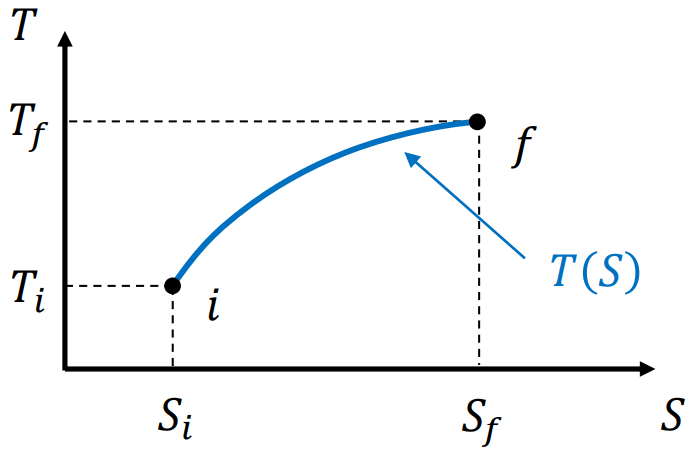
\includegraphics[height=3cm]{../L03/img8.PNG}
\end{center}
Per una trasformazione \textbf{ciclica} e \textbf{internamente reversibile}, le aree incluse nelle curve chiuse rappresentative del ciclo nei diagrammi P-V e T-S sono \textbf{uguali}, essendo, per il primo principio $L^\rightarrow  = Q^\leftarrow $
\begin{center}
    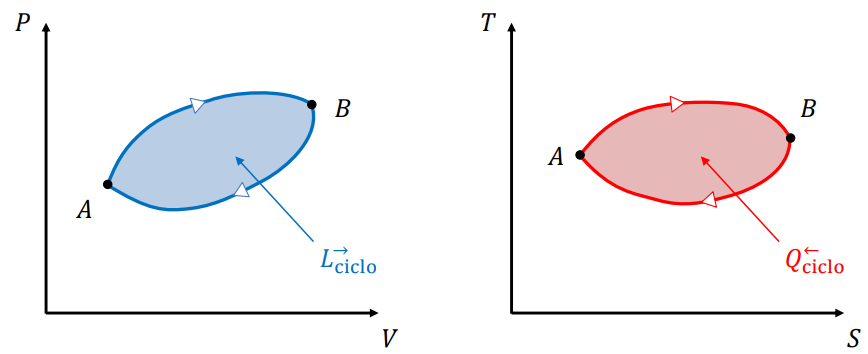
\includegraphics[height=3cm]{../L03/img9.PNG}
\end{center}
Nel piano T-S (o T-s) tutte le \textbf{politropiche} sono rappresentate da \textbf{esponenziali}:
\[
    T = T_0 e^{\frac{s-s_0}{c_x}}
\]
\begin{itemize}
    \item \textbf{Isoterme}: avendo $c_x = \infty$, sono \textbf{rette orizzontali} e così, per il \textbf{gas ideale}, anche le isoentalpiche dato che $h = h(T)$.
    \item \textbf{Adiabatiche reversibili (isoentalpiche)} invece sono \textbf{rette verticali} visto che $c_x = 0$.
    \item \textbf{Isocore}, essendo $c_V< c_P$ sono \textbf{più ripide} delle \textbf{isobare}.
\end{itemize}
\begin{center}
    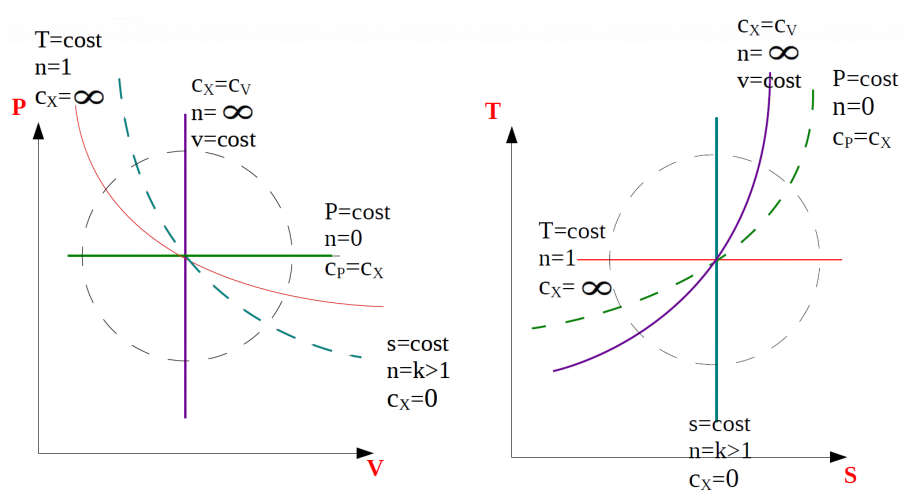
\includegraphics[height=5cm]{../L03/img10.PNG}
\end{center}
\subsection{Calcolo di grandezze termodinamiche ($u, h, s, l, q$)}
Per il calcolo dell'\textbf{energia interna}:
\begin{itemize}
    \item Per i \textbf{gas perfetti}: $\Delta u = c_v \Delta T$
    \item Per i \textbf{liquidi (e solidi) incomprimibili perfetti} ($v = costante$): $\Delta u = c \Delta T$
\end{itemize}
\ \newline
\newline
Per il calcolo dell'\textbf{entalpia}:
\begin{itemize}
    \item Per i \textbf{gas perfetti}: $\Delta h = c_P \Delta T$
\end{itemize}
\ \newline
\newline
Per il calcolo di \textbf{lavoro} e \textbf{calore} per \textbf{sistemi chiusi}, \textbf{determinate trasformazioni} e \textbf{GAS PERFETTI}:
\begin{center}
    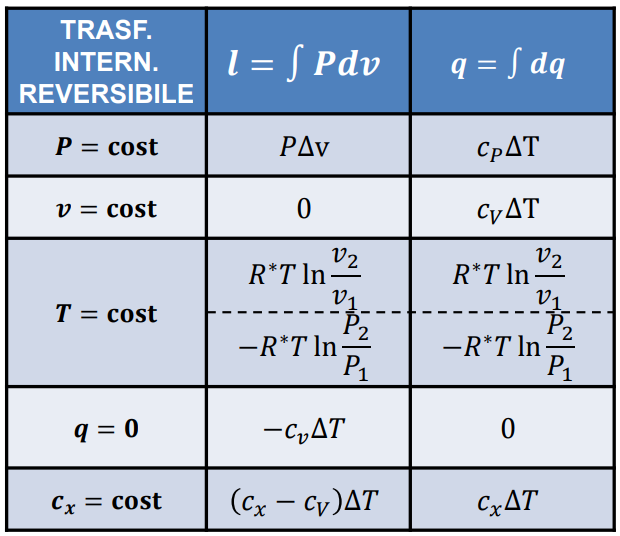
\includegraphics[height=7cm]{../L03/img11.PNG}
\end{center}
\ \newline
Per il calcolo dell'\textbf{entropia}:
\begin{itemize}
    \item Per un \textbf{generico sistema}: $\delta s = \frac{du}{T} + \frac{P}{T} dv$
    \item Per \textbf{gas ideali}: $ds = c_V \frac{dT}{T} + R^* \frac{dv}{v}$
    \item per \textbf{gas perfetti} ($c_V = costante$ e $c_P = costante$) possiamo integrare l'espressione e otteniamo: \newline
    \[
        \begin{matrix}
            \Delta s = s_2-s_1 &= c_V ln \frac{T_2}{T_1} + R^* ln \frac{v_2}{v_1} =\\
            \ \\
            &= c_P ln \frac{T_2}{T_1} - R^* ln \frac{P_2}{P_1} =\\
            \ \\
            &= c_P ln \frac{v_2}{v_1} + c_V ln \frac{P_2}{P_1}
        \end{matrix}
    \]
    \item per \textbf{liquidi (e solidi) incomprimibili perfetti} ($v = costante$): 
    \[
        \Delta s = s_2-s_1 = c ln \frac{T_2}{T_1}
    \]
\end{itemize}